\section{Pressure driven flows}
In order to induce flow in a system, it is common to apply a pressure gradient. A constant pressure gradient means that there acts a nonzero net force on any volume element $dV$ in the system. There might be regions where the net force \textit{is} zero, but on average, the simulated substance feels a force. In continuum models, the pressure, and hence pressure gradients, is often incorporated as boundary conditions where pressure is specified at given points. In particle models like DSMC, pressure must be defined through statistical mechanics and is actually not a required property. This is fairly obvious, because the knowledge of a consept like pressure should not change the rules of physics. The universe itself does not care about whether or not we have figured out what pressure is, but it is a convenient mathematical tool for us.

\subsection{What is pressure?}
The usual definition of pressure is the one from classical mechanics; force per area
\begin{align}
	P = \frac{F}{A}.
\end{align}
In statistical mechanics, the pressure is defined in a statistical manner through the entropy
\begin{align}
	P = T\left(\dpart{S}{V}\right)_{U,N},
\end{align}
which is the mathematical way to say \textit{pressure is the thing that is equal in two systems if they can exchange volume}. 

\subsection{Acceleration-driven flow}
We will use the ideas of continuum mechanics to derive a relation between the pressure gradient $\nabla P$ and a constant force $F$ (often called gravity), where the latter will be used to induce flow in the DSMC-algorithm. We look at a volume element of size $\Delta x\Delta y\Delta z$ in a channel with a continuous fluid and a pressure gradient in the $x$-direction, see figure \ref{fig:pressure_gravity_equivalent}. The force acting on the volume element from the pressure gradient is
\begin{align}
	F_x = P_1\Delta y\Delta z - P_2\Delta y\Delta z = \Delta y\Delta z\Delta P,
\end{align}
where $\Delta P = P_1 - P_2$. We aim to find a constant force $F_x=ma_x$ being equivalent to that of the pressure difference. With an applied acceleration $g$, the force is then
\begin{align}
	F_x = mg = \rho_m \Delta V g = \Delta y\Delta z\Delta P = \Delta V \frac{P}{\Delta x},
\end{align}
which gives the relation
\begin{align}
	g = \frac{P}{\rho_m\Delta x}.
\end{align}
This is the approach we have used to induce flow in the DSMC code, and the implementation is shown in listing \ref{lst:acceleration_driven_flow}.
\begin{lstlisting}[caption=Acceleration of particles in the DSMC code., label=lst:acceleration_driven_flow]
void System::accelerate(double acceleration, int flow_direction) {
    for(int n=0;n<num_molecules;n++) {
        v.at(3*n+flow_direction) += acceleration;
    }
}
\end{lstlisting}

\subsection{Limitations}
One problem with this approach appears if the path through a system has larger parts in the opposite direction of the pressure difference, see figure \ref{fig:gravity_problem}. If the system is driven by a real pressure difference, the net force on a volume element in the gray area would differ both in magnitude and direction.
\begin{figure}[h]
\begin{center}
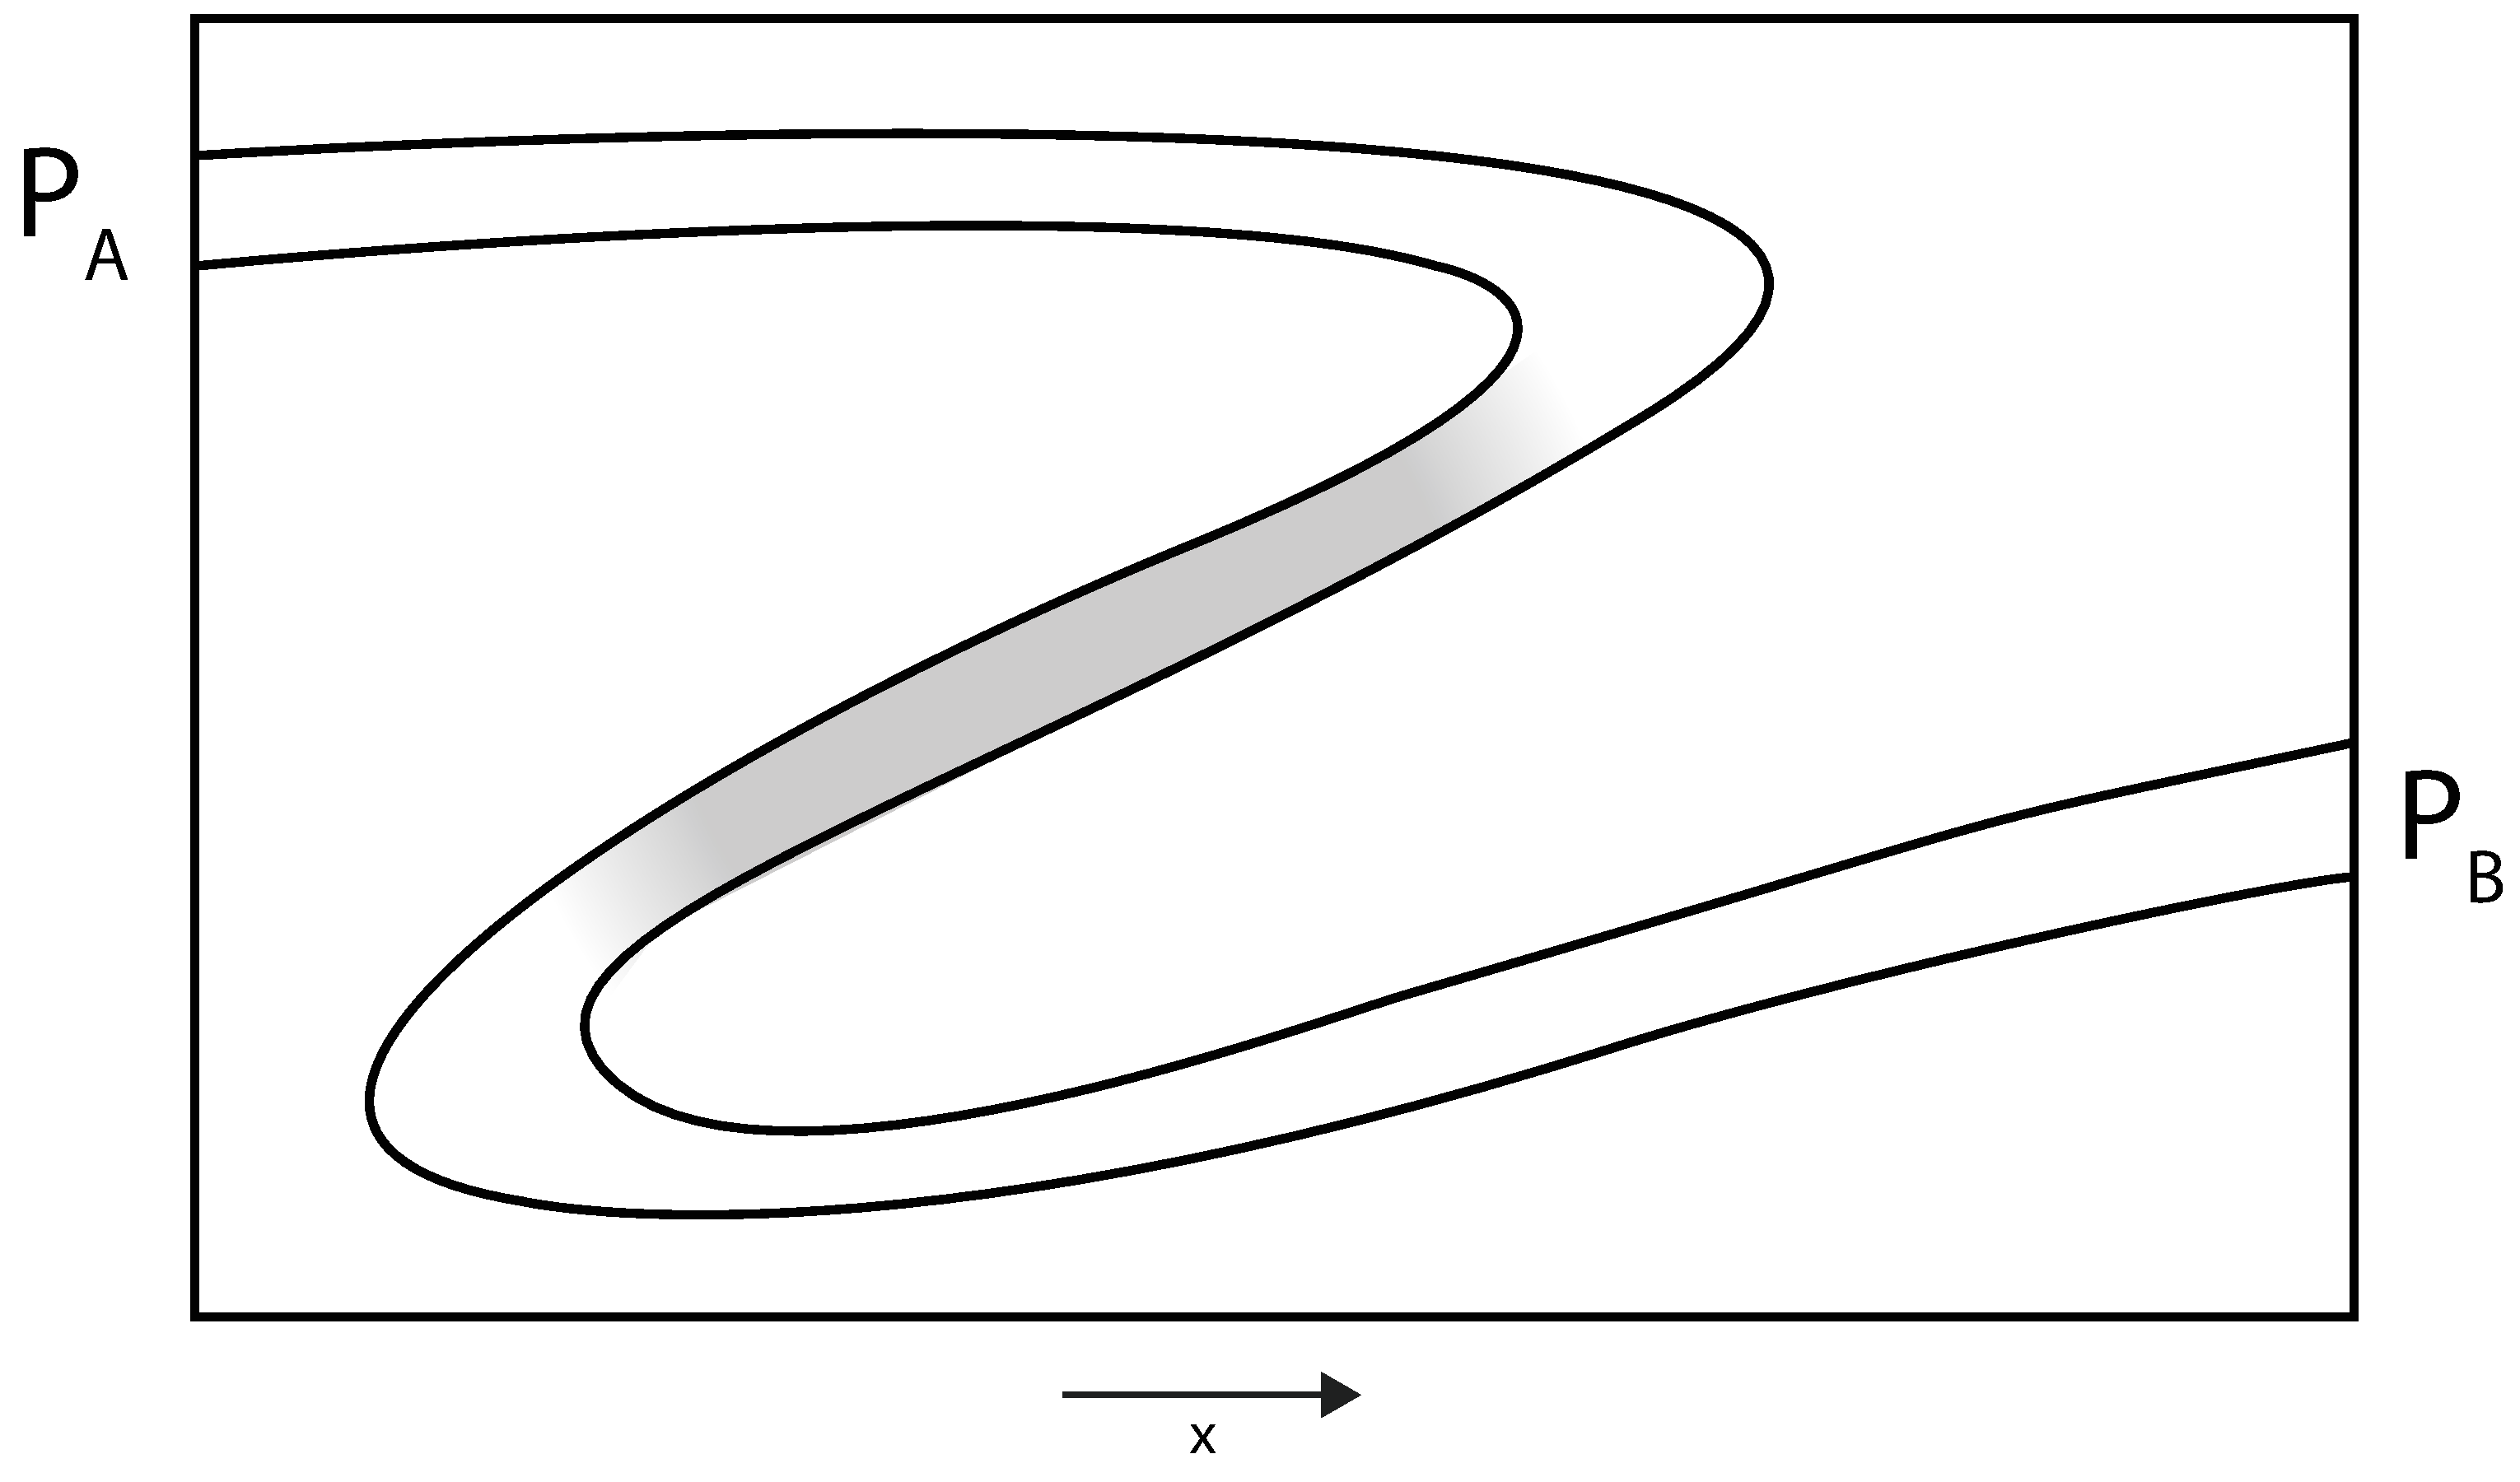
\includegraphics[width=0.7\textwidth, trim=0cm 0cm 0cm 0cm, clip]{DSMC/figures/gravity_problem.eps}
\label{fig:gravity_problem}
\end{center}
\caption{Acceleration-driven flows will not reproduce correct results when the gas in a large part (marked gray) of the channel will flow in the opposite direction of the pressure gradient.}
\end{figure}
